\section{Experiments}
\label{sec:experiments}

\subsection{Synthetic Gaussians}
We compare Euc-PD, WFR, WIFT, and MSIP on one- and two-dimensional Gaussian targets over $1000$ iterations, with RBF length scale $1$, $\alpha=1$, $\beta=0.5$, and $\tau\in\{0.01,0.1,1\}$. WIFT uses the explicit-Euler weight update. In the one-dimensional setting, $\pi=\mathcal{N}(1,0.7^2)$ and $N=100$ particles; Euc-PD, WFR, and WIFT start from an equally spaced grid on $[-2,2]$, whereas MSIP samples its initial particles uniformly on this interval. All four methods use the RBF kernel in this setting, without weight projection. In two dimensions, $\pi=\mathcal{N}(\bm{0},I_2)$ and $N=20$ particles, with close and far initial distributions $\mathcal{N}((1,1),I_2)$ and $\mathcal{N}((9,9),I_2)$. Euc-PD, WFR, and WIFT use the linear-plus-RBF kernel with unit linear coefficient and simplex-projected weights, whereas the upstream MSIP implementation uses the RBF kernel.

Figure~\ref{fig:all_mmd} reports pointwise median MMD across seeds $42$--$46$, with capped error bars every $100$ iterations showing the sample standard deviation divided by $\sqrt{n}$ for the $n$ successful seeds. These bars describe across-seed variability about the median; they are not confidence intervals for the median. No smoothing is applied. The deterministic one-dimensional initialization gives zero variability for Euc-PD, WFR, and WIFT. MSIP has five and four successful seeds in one dimension at $\tau=0.01$ and $\tau=0.1$, respectively, five at both step sizes under close initialization, and three and four under far initialization. No MSIP trajectory at $\tau=1$ is included. All other plotted settings have five complete seeds. Appendix~\ref{app:distant-initialization} provides particle trajectories for seed $42$.

\begin{figure*}[t]
    \centering
    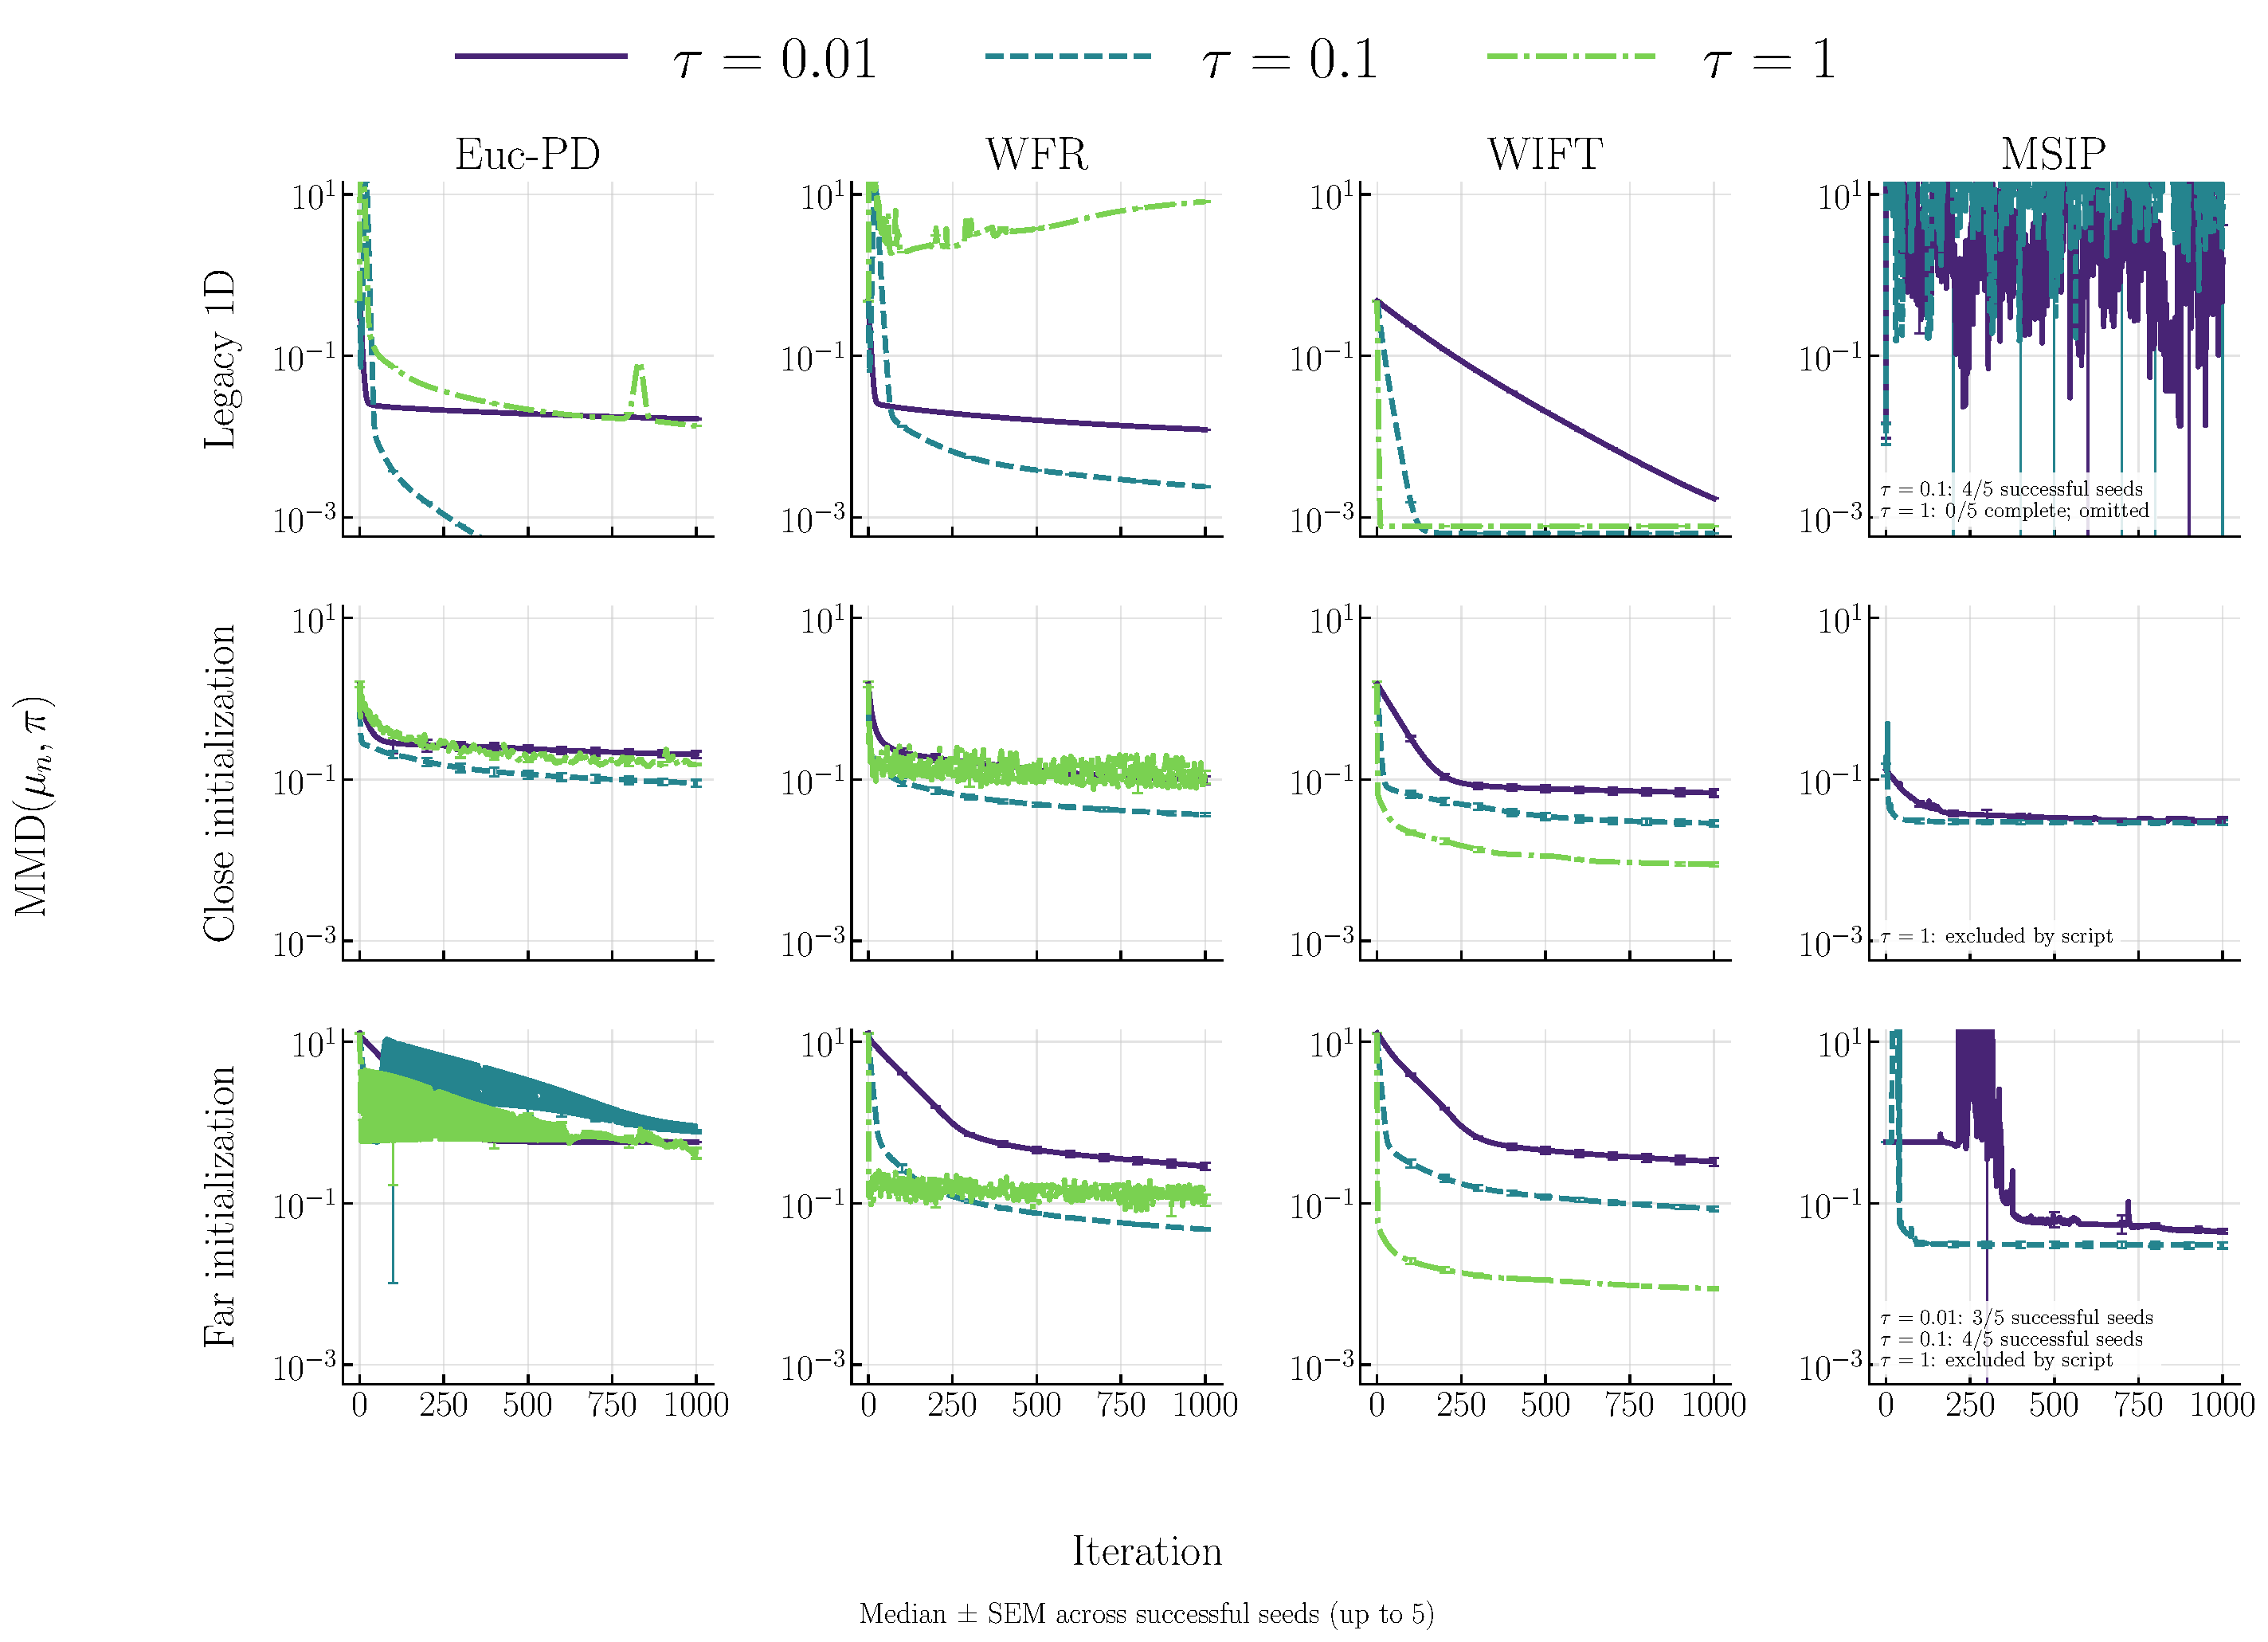
\includegraphics[width=1.0\linewidth]{figures/all_mmd_trajectories.pdf}
    \caption{\textbf{Gaussian synthetic.} Median MMD trajectories for Euc-PD, WFR, WIFT, and MSIP. Rows show the one-dimensional target, close two-dimensional initialization, and far two-dimensional initialization. Capped error bars show across-seed SEM for up to five successful seeds; reduced MSIP counts are annotated. All panels share logarithmic y-axis limits derived from the WIFT medians and error bars.}
    \label{fig:all_mmd}
\end{figure*}


\subsection{Mean-field student-teacher neural networks}
We next test the particle geometries in a nonlinear regression problem. For an input $z\in\R^d$, each particle is an augmented neuron parameter $\theta^{(i)}=(a^{(i)},b^{(i)})\in\R^{d+1}$, and the student network is $f_{\mu_N}(z)=\sum_{i=1}^N w^{(i)}a^{(i)}\sigma(z^\top b^{(i)})$. Keeping the signed output coefficient $a^{(i)}$ inside the particle allows the measure weights $w^{(i)}$ to remain nonnegative. The teacher $f_\star$ has the same two-layer mean-field form with $M$ hidden features and uniform measure weights $1/M$. For fixed inputs $z_1,\ldots,z_L$, we use the empirical neuron kernel $k(\theta,\theta')=L^{-1}\sum_{\ell=1}^L a a'\sigma(z_\ell^\top b)\sigma(z_\ell^\top b')$. With residuals $r_\ell=f_{\mu_N}(z_\ell)-f_\star(z_\ell)$, the resulting MMD is exactly the root-mean-square student--teacher mismatch:
\begin{align*}
    \mmd^2(\mu_N,\pi_M)
    &= \frac{1}{L}\sum_{\ell=1}^L r_\ell^2.
\end{align*}

We use ReLU activation, dimensions $d\in\{10,50\}$, $N=100$ student particles, teacher widths $M\in\{50,200\}$, and $L=2048$ fixed inputs. The inputs follow $\mathcal{N}(\bm{0},I_d/d)$, while the teacher hidden parameters and initial student hidden parameters follow $\mathcal{N}(\bm{0},I_d)$. The teacher output parameters follow $\mathcal{N}(0,M)$, so after multiplication by the uniform teacher weight $1/M$, their effective coefficients follow $\mathcal{N}(0,1/M)$. We initialize the student output parameters at $a^{(i)}=1$ and the measure weights at $w^{(i)}=1/N$. We vary the student seed over $42$--$46$ while fixing the teacher and input seeds to $123$ and $456$, respectively, use $\alpha=1$ and $\beta=0.5$, project the particle weights onto the probability simplex, use the explicit-Euler weight update for WIFT, and run every method for $1000$ iterations.

Figure~\ref{fig:mean-field-nn} compares $\tau\in\{0.01,0.1,1\}$. To make the method panels directly comparable, every panel uses the same logarithmic y-axis limits, derived from the WIFT medians and error bars across all four settings. Lines show pointwise medians over five completed student initializations, with capped across-seed SEM bars every $100$ iterations as in the Gaussian experiments.

\begin{figure*}[t]
    \centering
    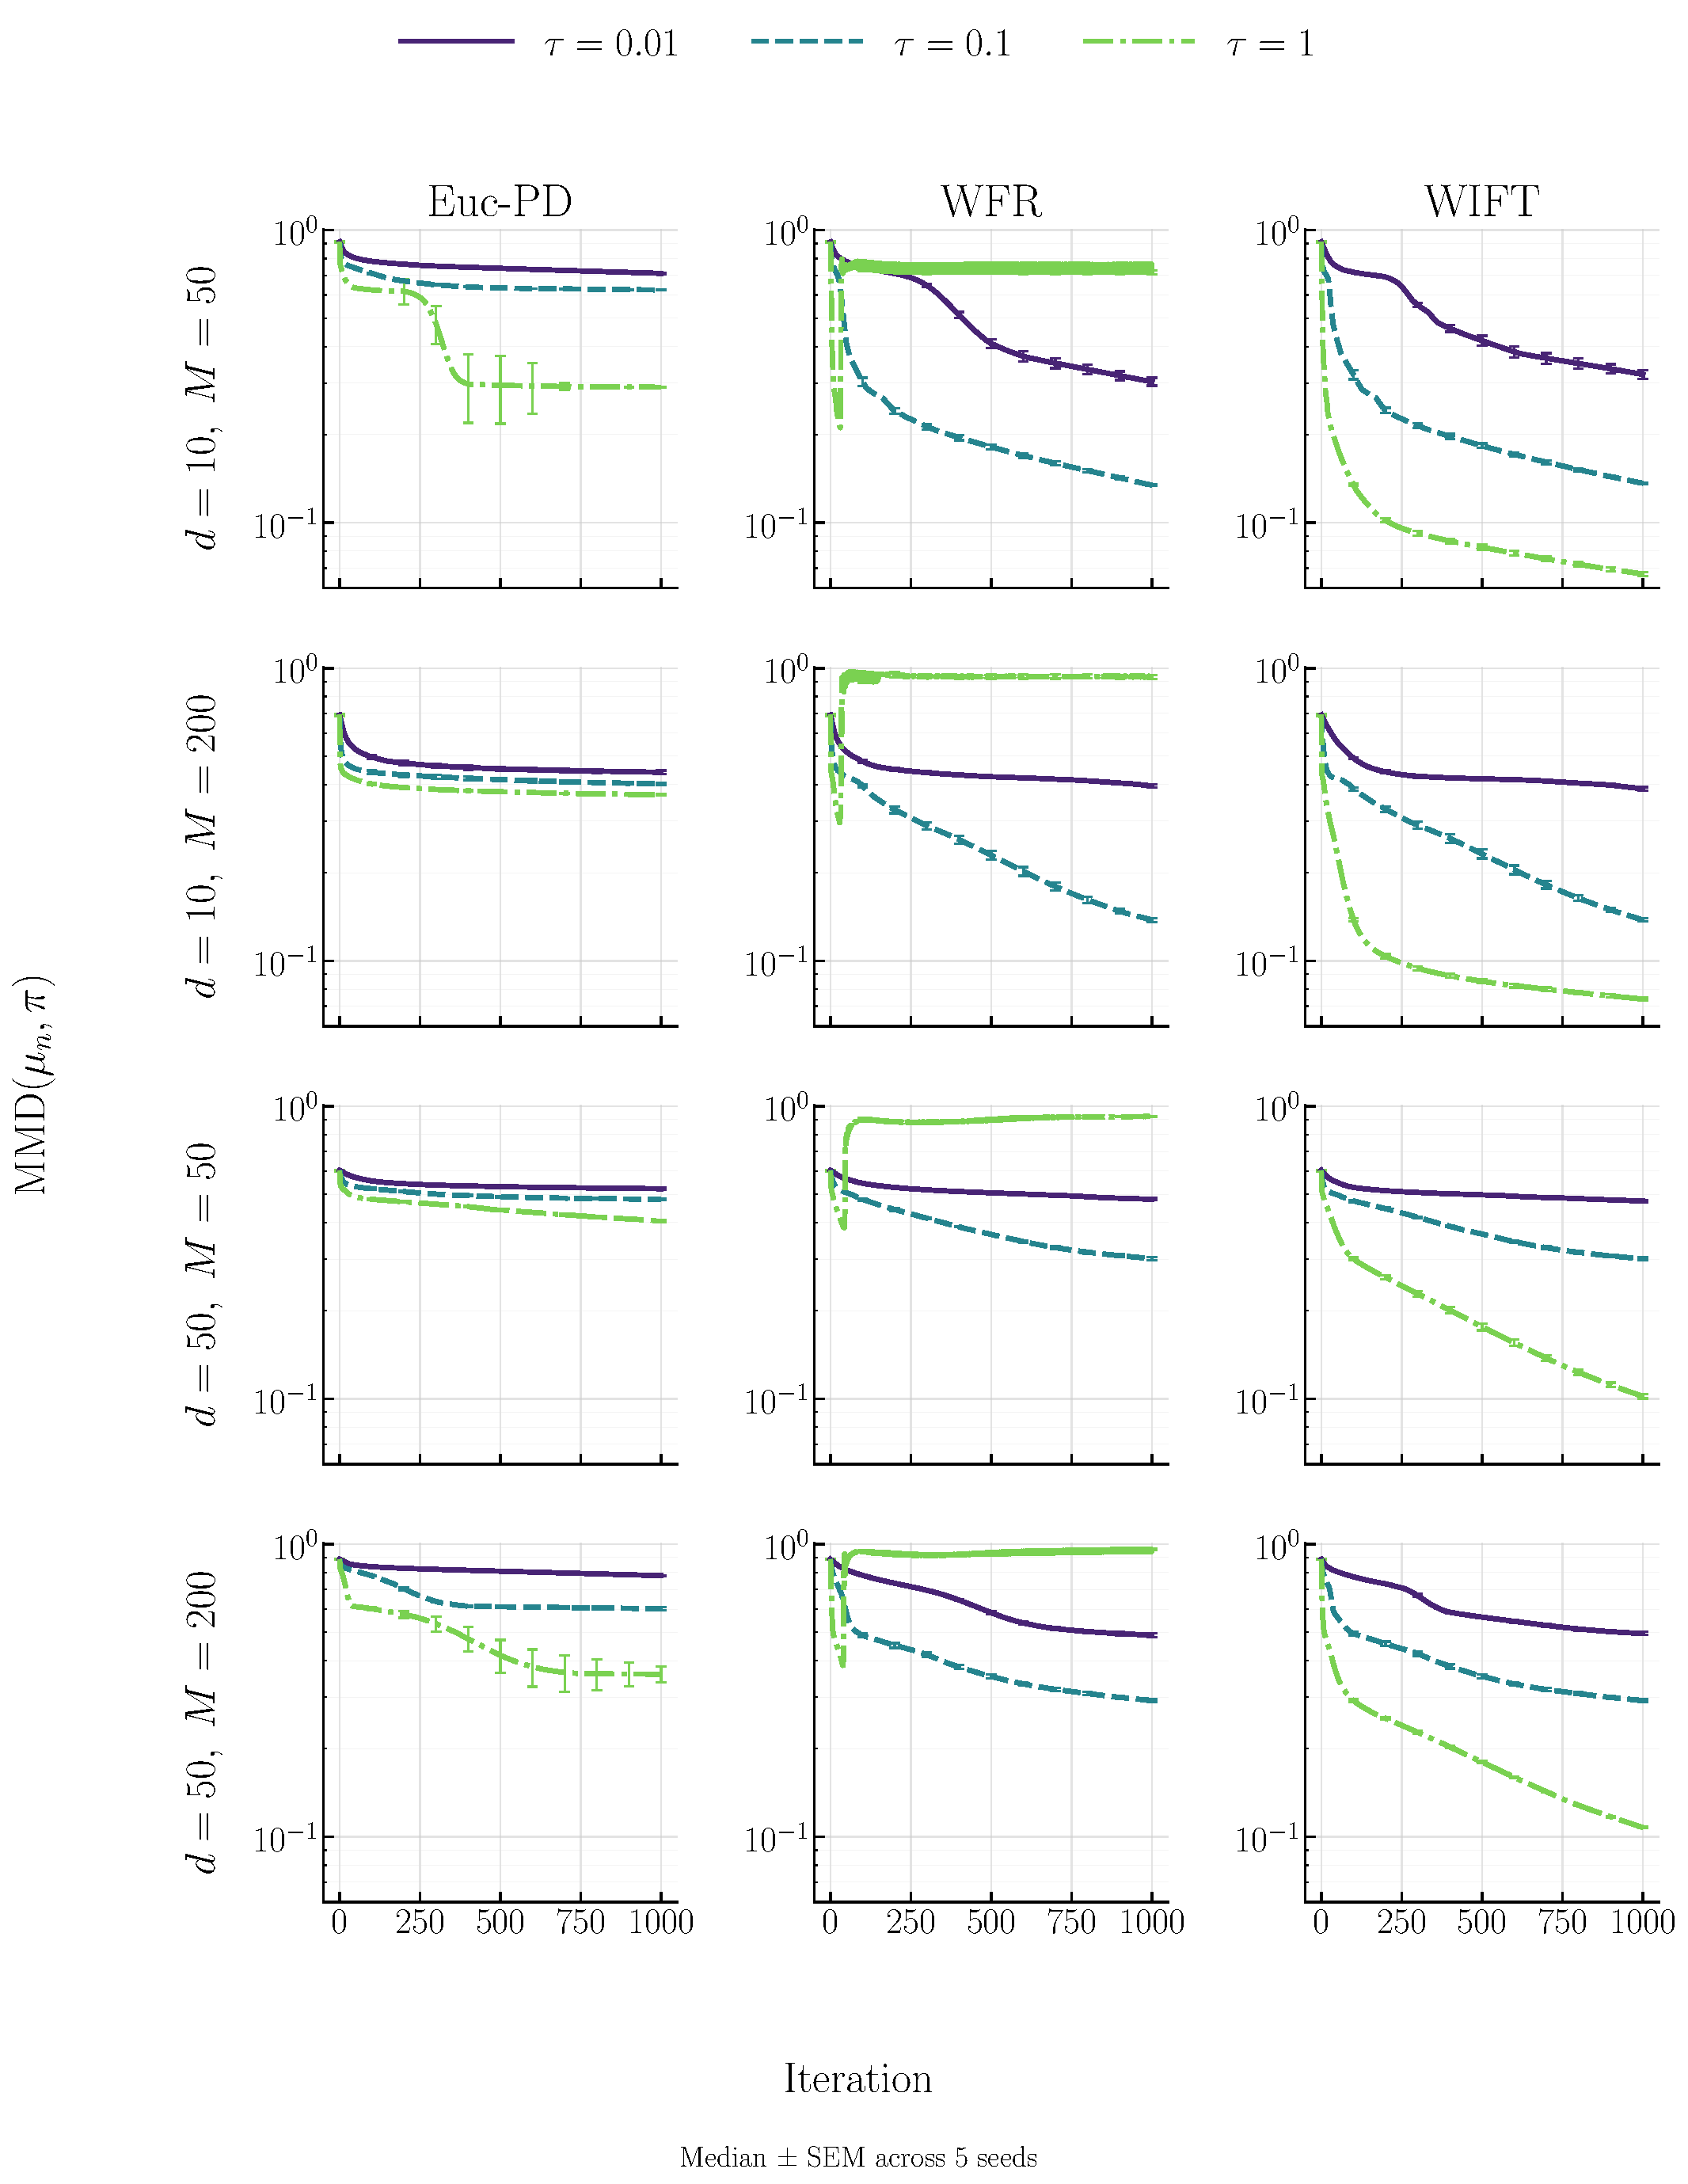
\includegraphics[width=0.94\linewidth]{figures/mean_field_nn_trajectories.pdf}
    \caption{\textbf{Mean-field ReLU student--teacher networks.} Median MMD trajectories for Euc-PD, WFR, and WIFT over $1000$ iterations with $N=100$ student particles and $L=2048$ fixed inputs. Rows show $(d,M)=(10,50),(10,200),(50,50),(50,200)$. Capped error bars show across-seed SEM over five student initializations. All panels share logarithmic y-axis limits derived from the WIFT medians and error bars.}
    \label{fig:mean-field-nn}
\end{figure*}

WIFT attains its lowest final median MMD at $\tau=1$ in all four settings, reaching $0.0668$, $0.0740$, $0.1019$, and $0.1076$ in row order. The best final medians over the tested step sizes are $0.2906$, $0.3696$, $0.4058$, and $0.3597$ for Euc-PD, and $0.1346$, $0.1379$, $0.3014$, and $0.2925$ for WFR. Euc-PD performs best at $\tau=1$ and WFR at $\tau=0.1$ in each setting.
